\documentclass[10 pt]{article}

\usepackage[OT1, OT2]{fontenc}
\newcommand{\Lat}{\fontencoding{OT1}\selectfont}
%\usepackage[english, serbian]{babel}
\usepackage[top= 27mm, bottom=27mm, left=25mm, right=25mm]{geometry}
%\usepackage{amsmath}
%\usepackage{amssymb}
%\usepackage{amsthm}
\usepackage{graphicx}
%\usepackage{subfig}
\usepackage{hyperref}
\usepackage{indentfirst}

\renewcommand*\contentsname{Sadrzhaj:}
\renewcommand{\figurename}{Slika}
\renewcommand{\refname}{Literatura}

\hypersetup{
    colorlinks=true,
    linktoc=all,
    linkcolor=blue,
}


\title{\vspace*{\fill}\huge{\textbf{Grupni projektni rad\\ 
		\vspace{10 pt} Informacioni sistem za iznoshenje smec1a}}}
\date{}
\author{}

\begin{document}

\maketitle	

\
\\[270 pt]
\
\begin{flushleft}
	Studenti:\hspace{260 pt} Predmet: Informacioni sistemi\\ 
	Miroslav Mishljenovic1\hspace{197 pt} Profesor: Sasha Malkov\\
	Filip Lazic1\hspace{244 pt} Asistent: Aleksandra Kocic1\\
	Nemanja Antic1\\
	Marija Mijailoic1 
 \end{flushleft}

 \
 \\[50 pt]
 \
\begin{center}
  Univerzitet u Beogradu, Matematichki fakultet
  \\ novembar 2017. godine
\end{center}

\thispagestyle{empty}

\newpage
\tableofcontents

\newpage
\section{Uvod}

\subsection{Kratak opis sistema}
\setlength{\parindent}{30pt} Sistem za iznoshenje otpada funkcionishe tako shto se razne vrste otpada odlazhu na za tu vrstu predvidjen nachin. Sistem omoguc1ava iznoshenje razlichitih vrsta otpada kao shto su gradjevinski, reciklazhni, elektrichni, itd … Takodje sistem omoguc1ava prac1enje radnika na terenu koji rade na procesu iznoshenja i odlaganja otpada(radnici, vozachi…). Deo sistema c1e se baviti naplac1ivanjem usluga. U okviru sistem podrazumeva da postoji sistem za reciklazhu, i magacin za skladishtenje otpada.  

\subsection{Akteri}
	\begin{enumerate}
		\item
			\textit{\textbf{Klijent}} je subjekat chiji se otpad odlazhe. Mozhe biti redovan pretplatnik usluga iznoshenja smec1a ili firma koja trazhi ekspilicitno iznochenje otpada(naplac1uje se po posebnom sistemu naplate).
		\item 
			\textit{\textbf{Dispecher}} prikuplja zahteve klijenata i u skladu sa resursima kojima sluzhba raspolazhe u tom trenutku rasporedjuje zahteve odredjenom koordinatoru u zavisnosti od toga koja je vrsta otpada u pitanju.
		\item 
			\textit{\textbf{Koordinator za hemijski otpad}} koordinira procesom odlaganja hemijskog otpada. Upravlja klasifikacijom, odlaganjem i sprovodi sistem naplate.
		\item 
			\textit{\textbf{Koordinator za reciklazhni otpad}} koordinira procesom odlaganja reciklazhnog otpada. Upravlja klasifikacijom, odlaganjem i sprovodi sistem naplate.
		\item 
			\textit{\textbf{Koordinator za komunalni otpad}} koordinira procesom odlaganja ostalog otpada. Upravlja klasifikacijom, odlaganjem i sprovodi sistem naplate. 	
		\item 
			\textit{\textbf{Radnici}} sprovode zadatke koje postavlja odgovarajuc1i koordinator. Mozhe biti vozach, radnik na rukovanju kontejnerima, itd…
		\item 
			\textit{\textbf{Magacioner}} skladishti otpad u magacin. 
	\end{enumerate}


\section{Analiza sistema}
\setlength{\parindent}{30pt} Postojec1i sistem sadrzhi prevelik broj zaposlenih u administraciji. Ovaj sistem je napravljen sa pokushajem da smanji broj ljudi u administraciji i sistem uchini jednako efikasnim. Takodje, u odnosu na prethodni sistem nash podrazumeva i savremeniju opremu za rad. Prikaz informaciong sistema dat je na sliciX. 

\subsection{Dijagram celog sistema}
\begin{center}
	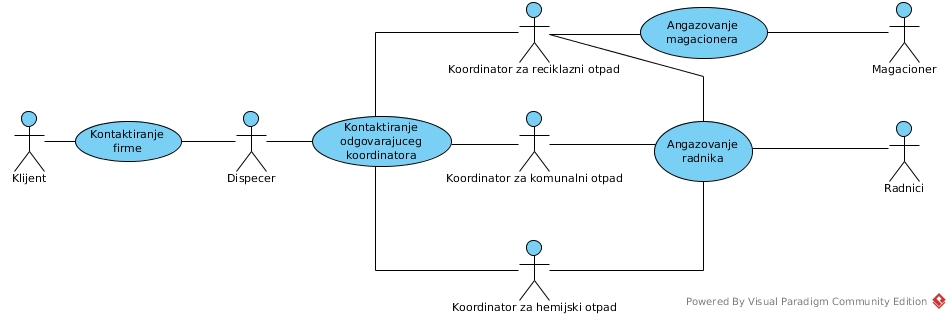
\includegraphics[width=15cm,height=15cm,keepaspectratio]{slike/DijagramCelogSistema}\\
	%Opis	
\end{center}

\section{Sluchajevi upotrebe}


\subsection{Dispecher kontaktira odgovarajuc1eg koordinatora}

\begin{itemize}
	\item \textit{Kratak opis} - Dispecher dobija zahteve od klijenta i shalje odgovarajuc1em koordinatoru
	\item \textit{Uchesnici} \\
		\begin{enumerate}
			\item Klijent
			\item Dispecher
			\item Koordinator
		\end{enumerate}
	\item \textit{Preduslovi} - Klijent je uspeshno kontaktirao dispechera
	\item \textit{Postuslovi} - Dispecher je uspeshno poslao zahtev odgovarajuc1em koordinatoru
	\item \textit{Osnovni tok} - Klijent obaveshtava dispechera preko:\\
		\begin{itemize}
			\item online formulara
			\item pozivom
		\end{itemize}
	\item \textit{Alternativni tokovi} - Klijent nije adekvatno popunio online formular. Dispecher kontaktirao klijenta
	\item \textit{Podtokovi} - Nema
	\item \textit{Specijalni zahtevi} - Nema
	\item \textit{Dodatne informacije} - Nema
\end{itemize}

\subsection{Hemijski otpad}
\begin{itemize}
	\item \textit{Kratak opis} - 
	\item \textit{Uchesnici} -
	\item \textit{Preduslovi} -
	\item \textit{Postuslovi} - 
	\item \textit{Osnovni tok} - 
	\item \textit{Alternativni tokovi} - 
	\item \textit{Podtokovi} - 
	\item \textit{Specijalni zahtevi} - 
	\item \textit{Dodatne informacije} - 
\end{itemize}


\subsection{Reciklazhni otpad}

\begin{itemize}
	\item \textit{Kratak opis} - 
	\item \textit{Uchesnici} -
	\item \textit{Preduslovi} -
	\item \textit{Postuslovi} - 
	\item \textit{Osnovni tok} - 
	\item \textit{Alternativni tokovi} - 
	\item \textit{Podtokovi} - 
	\item \textit{Specijalni zahtevi} - 
	\item \textit{Dodatne informacije} - 
\end{itemize}

\subsection{Komunalni otpad}

\begin{itemize}
	\item \textit{Kratak opis} - 
	\item \textit{Uchesnici} -
	\item \textit{Preduslovi} -
	\item \textit{Postuslovi} - 
	\item \textit{Osnovni tok} - 
	\item \textit{Alternativni tokovi} - 
	\item \textit{Podtokovi} - 
	\item \textit{Specijalni zahtevi} - 
	\item \textit{Dodatne informacije} - 
\end{itemize}

\section{Administracija sistema}

\section{Klase podataka}

\section{Prototipovi}
\section{Zakljuchak}
\section{Reference}

\end{document} 